\documentclass{beamer}
\usetheme{Warsaw}


\title[DevOps as culture]{DevOps as culture: what the history of DevOps can teach us about its implementation}
\author{Jacob Archambault}
\institute[TCS]{Tata Consultancy Services}
\AtBeginSubsection[]
{
	\begin{frame}<beamer>{Outline}
		\tableofcontents[currentsection, currentsubsection]
	\end{frame}
}

\begin{document}
	\begin{frame}[plain]
		\titlepage
	\end{frame}
	\begin{frame}{Outline}
		\tableofcontents[pausesections]
		% You might wish to add the option [pausesections]
	\end{frame}
	\section{Challenges for DevOps today}
	\subsection{For developers and enquirers}
	\begin{frame}{DevOps challenges: developers and inquirers}
		\begin{itemize}\item 	Overwhelming amount of toolchain growth \pause
			\item added complexity \pause
			\item doesn't feel like I'm going faster or solving problems.\pause
			\item Meaning of DevOps is opaque \pause
			\begin{itemize}
				\item CI/CD pipeline management \pause
				\item Docker, Kubernetes, Terraform \pause
				\item Identity and access permissions \pause
				\item AWS, Azure, Google Cloud 
			\end{itemize}
		\end{itemize}
	\end{frame}
	\subsection{For business}
	\begin{frame}{DevOps challenges: business}
		\begin{itemize}
			\item DevOps engineers are among the highest paid positions outside of management
			\pause
			\item Not using DevOps technologies poses a flight risk \pause
		\end{itemize}
	\end{frame}
	\subsection{Common challenges}
	\begin{frame}{DevOps challenges: avoiding a worst-of-all-worlds scenario}
		\begin{itemize}
			\item increased operating costs from hiring more experienced developers \pause
			\item added unnecessary complexity in our dev stack \pause
			\item restricted the freedom of developers to get work done \pause
			\item forfeited ownership of our infrastructure \pause 
			\item rebranded our operations team
		\end{itemize}
	\end{frame}
	\section{A short history of DevOps}
	\subsection{Its roots}
	\subsubsection{Throughput}
	\begin{frame}{Just-in-time manufacturing and Goldratt's theory of constraints}
		\begin{itemize}
			\item Increase: throughput \pause
			\item Decrease: \pause
			\begin{itemize}
				\item operating costs \pause
				\item inventory \pause
				\item scrap \pause
			\end{itemize}
			\item Remove bottlenecks
		\end{itemize}
	\end{frame}
	\begin{frame}{Goldratt's theory of constraints (cont.)}
		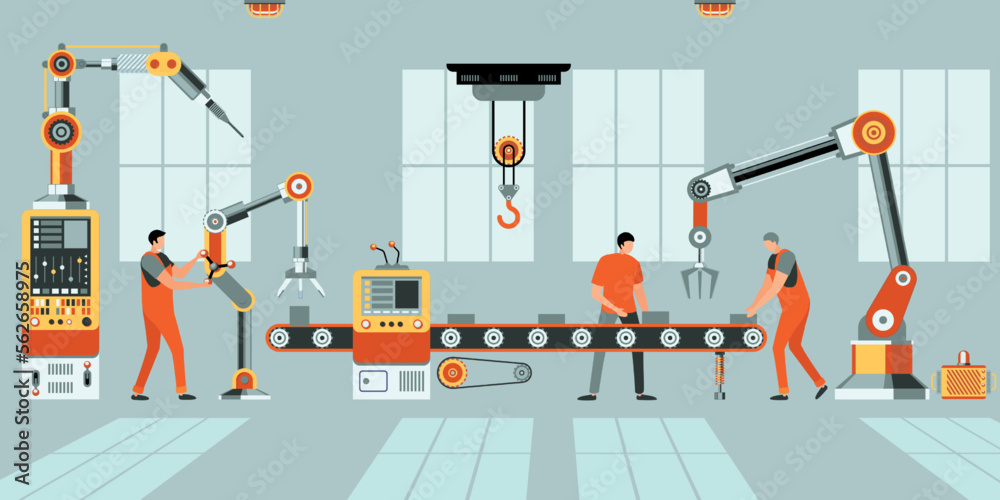
\includegraphics{assemblyline}
	\end{frame}
	\subsubsection{Communication}
	\begin{frame}{1967: Conway's law}
		\begin{quote}
			`Organizations which design systems [...] are constrained to produce designs which are copies of the communication structures of these organizations.' - Melvin Conway, `How do Committees Invent?' Datamation, 1967
		\end{quote}
	\end{frame}
	\begin{frame}{Conway's law: examples}
		\begin{itemize}
			\item `If you have four groups working on a compiler, you'll get a 4-pass compiler' - The New Hacker's Dictionary, 1996\pause
			\item front-end [devs] business layer [backend devs] monolithic database [DBA team] \pause
			\item a web api controller [manager]  delegates most business logic to business classes [developers] which are part of the same in-memory process [team], while serving as a single entry-point for wider cross-network [cross-team] communication.
		\end{itemize}
	\end{frame}
	\begin{frame}{1975: The Mythical Man Month, Fred Brooks}
		
		\begin{itemize}
			\item number of direct communication paths for $n$ individuals= $n(n-1)/2$
		\end{itemize}
		\begin{center}
			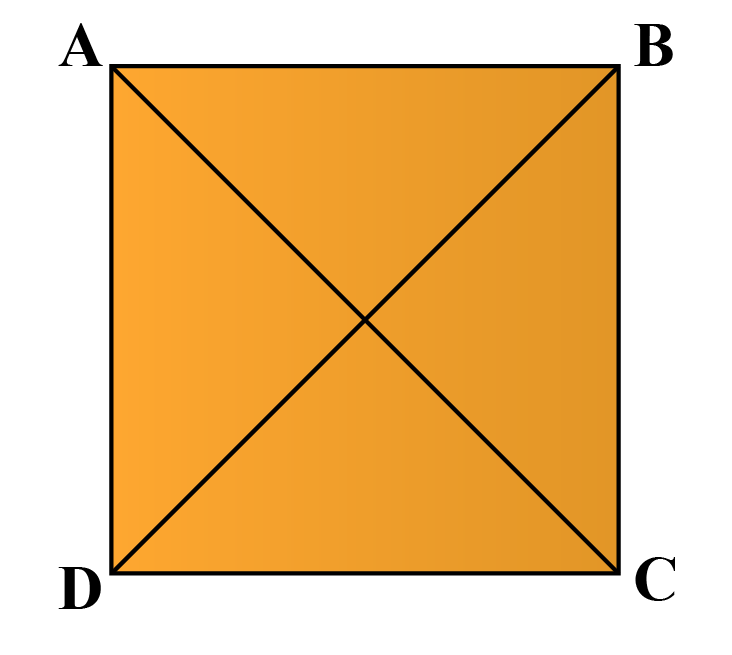
\includegraphics[width=.5\textwidth]{square}
		\end{center}
		
	\end{frame}
	\begin{frame}{1975: The Mythical Man Month, Fred Brooks}
		
		\begin{itemize}
			\item number of direct communication paths for $n$ individuals= $n(n-1)/2$
		\end{itemize}
		\begin{center}
			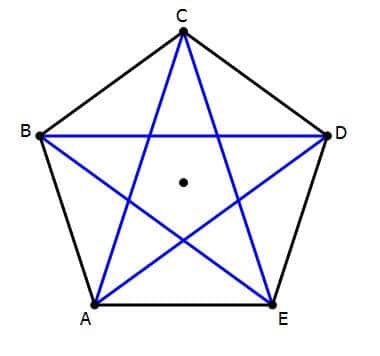
\includegraphics[width=.5\textwidth]{pentagon}
		\end{center}
		
	\end{frame}
	\begin{frame}{1975: The Mythical Man Month, Fred Brooks}
		
		\begin{itemize}
			\item number of direct communication paths for $n$ individuals= $n(n-1)/2$
		\end{itemize}
		\begin{center}
			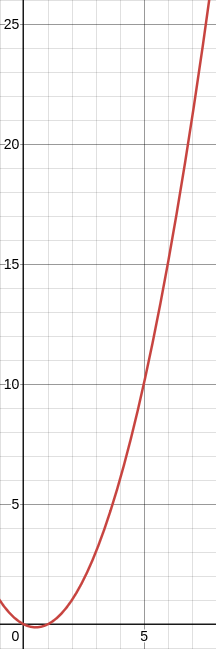
\includegraphics[width=.15\textwidth]{graph}
		\end{center}
	\end{frame}
	\begin{frame}{The Mythical Man Month, Fred Brooks (cont.)}
		\begin{itemize}
			\item corollary: adding more people to a project can lead not only to diminishing returns on delivery speed, but to objectively less work being completed
		\end{itemize}
	\end{frame}
	\subsection{Its emergence}
	\begin{frame}{DevOps: its beginning}
		\begin{itemize}
			\item Velocity Conference 2009: John Allspaw and Paul Hammond, "10+ Deploys Per Day: Dev and Ops Cooperation at Flickr" \pause
			\item Patrick Debois \href{https://youtu.be/EOveXZhJpr4}{DevOps Days 2009, Ghent, Belgium}
		\end{itemize}
	\end{frame}
	\subsection{Its growth}
	\subsubsection{DevOps Research and Assessment (DORA)}
	\begin{frame}{2013: The State of DevOps Report}
		\begin{enumerate}
			\item a series of surveys of over 36,000 professionals \pause
			\item Led by a PhD statistician, Nicole Forsgren, from 2013-2019 \pause
			\item Uses \emph{cluster analysis} to discover groupings - has no prior understanding of what counts as good or bad.
		\end{enumerate}
	\end{frame}
	\begin{frame}{The State of DevOps Report: throughput metrics}
		\begin{enumerate}
			\item lead time for changes \pause
			\item deployment frequency 
		\end{enumerate}
	\end{frame}
	\begin{frame}{The State of DevOps Report: stability metrics}
		\begin{enumerate}
			\item change failure rate \pause
			\item mean time to restore
		\end{enumerate}
	\end{frame}
	\begin{frame}{The State of DevOps Report: results}
		\begin{quote}
			`Astonishingly, these results demonstrate that there is no trade-off between improving performance and achieving higher levels of stability and quality. Rather, high performers do better at all of these measures. This is precisely what the Agile and Lean movements predict, but much dogma in our industry still rests on the false assumption that moving faster means \emph{trading off} against other performance goals, rather than enabling and reinforcing them.'  - Nicole Forsgren, Jez Humble, and Gene Kim, \emph{Accelerate} (2017), p. 14
		\end{quote}
	\end{frame}
	\section{DevOps anti-patterns and applications}
	\subsection{anti-pattern 1: local optimization}
	\begin{frame}{anti-pattern 1: local optimization}
		\begin{itemize}
			\item example 1: separate (DevOps, QA, operations, support) team \pause
			\item leads to bottlenecks \pause
			\item delays communication \pause
			\item punishes untracked work (e.g. thorough code reviews/dev testing, helping blocked colleagues)
		\end{itemize}
	\end{frame}
	\begin{frame}{anti-pattern 1 solution}
		\begin{itemize}
			\item cross-functional teams with `t-shaped' employees \pause
			\item guild system 
		\end{itemize}
	\end{frame}
	\subsection{Anti-pattern 2: Gandalf vs. the Balrog}
	\begin{frame}{Anti-pattern 2: Gandalf vs. the Balrog}
		\begin{center}
			
\includegraphics[width=.5\textwidth]{gandalf-balrog}
		\end{center}
	\end{frame}
	\begin{frame}{Anti-pattern 2: Gandalf vs. the Balrog}
		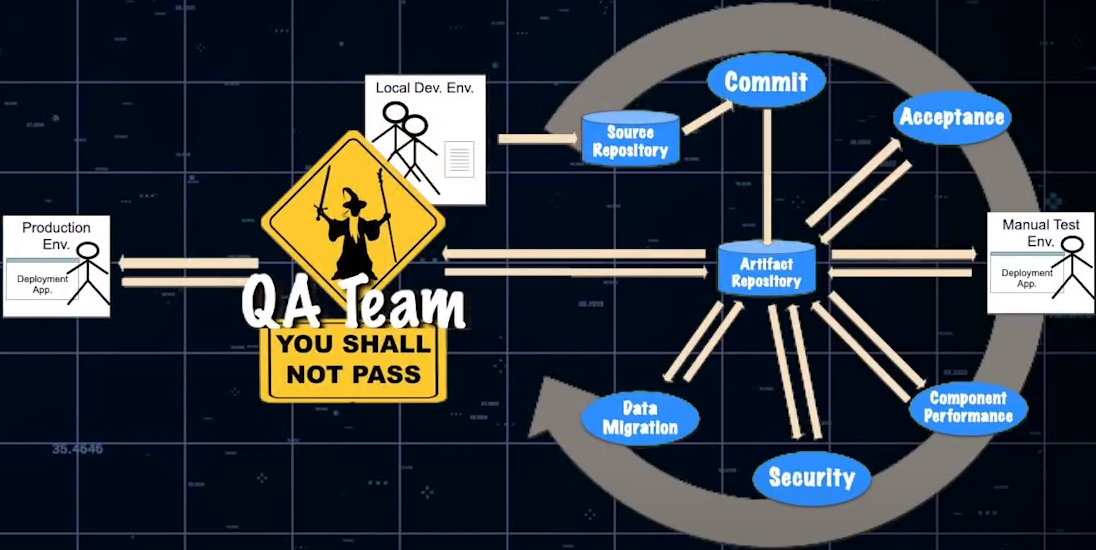
\includegraphics[width=\textwidth]{gandalf}
	\end{frame}
	\begin{frame}{anti-pattern 2: Gandalf vs. the Balrog}
		\begin{itemize}
			\item change approval boards \pause 
			\item pre-merge code reviews \pause 
			\item `bridge-to-nowhere' pipelines \pause
			\item these all increase lead time
		\end{itemize}
	\end{frame}
	\begin{frame}{anti-pattern 2 solutions: aggressively parallelize work}
		\begin{itemize}
			\item pair programming \pause 
			\item parallelized pipeline builds for `wide' pipelines \pause
			\item one build artifact for all pipeline stages \pause
			\item share responsibility
		\end{itemize}
	\end{frame}
	\section{Conclusion}
	\begin{frame}{Conclusion}
		\begin{enumerate}
			\item Reduce goal misalignment \pause
			\item stop people from waiting on each other \pause 
			\item work in small batches \pause
			\item That's mostly it
			
		\end{enumerate}
	\end{frame}
	\begin{frame}{Conclusion}
		\begin{quote}
			`DevOps is whatever you do to bridge friction created by silos, and all the rest is engineering' - Patrick Debois, Puppet State of DevOps report 2021
		\end{quote}
	\end{frame}
\end{document}
